In this chapter we will explore the mathematical structure of symmetry in the software synthesis process, mostly the work published in ~\cite{goens_iess15,goens_taco17,goens_scopes17,goens_tcad21}.
The material in this section makes use of concepts in group theory.
We assume the basic concepts as seen in any undergraduate course on group
theory, with the definitions of groups, actions and orbits.
A brief introduction, to the level required by this chapter, can be fonud in Appendix~\ref{appendix:groups}. 

\subsection{Architectures and Applications}

Intuitively, when we say an object is very symmetric we usually mean it has parts that are similar or identic, and the object looks identical (or similar) from multiple points of view.
In a symmetric face, for example, both the left and right sides of the face are similar. A hexagonal mosaic might look the same when seen from six different angles.
Mathematically, this is commonly modeled through transformations. A reflection along the vertical axis in a face, or rotations of $60^\circ$ in the heaxgon, both leave the object (mostly) unchanged.
We can do the same for hardware architectures, even heterogeneous ones.

For example, the Exynos~5 in the Odroid-XU4 has four identical Cortex A7\texttrademark, say $\PE_1,\ldots,\PE_4$ and four identical Cortex A15\texttrademark cores, say $\PE_5,\ldots,\PE_8$.
A transformation that swaps the cores $\PE_1$ and $\PE_2$ leaves the archtiecture topology unchanged, since the cores are identical. This is depicted in Figure~\ref{fig:exynos_symmetries}.
On the other hand, a transformation that swaps $\PE_1$ and $\PE_5$ does change the topology, since the cores are of different types. As can also be seen in Figure~\ref{fig:exynos_symmetries}.
\begin{figure}[h]
	\centering
\resizebox{0.3\textwidth}{!}{
   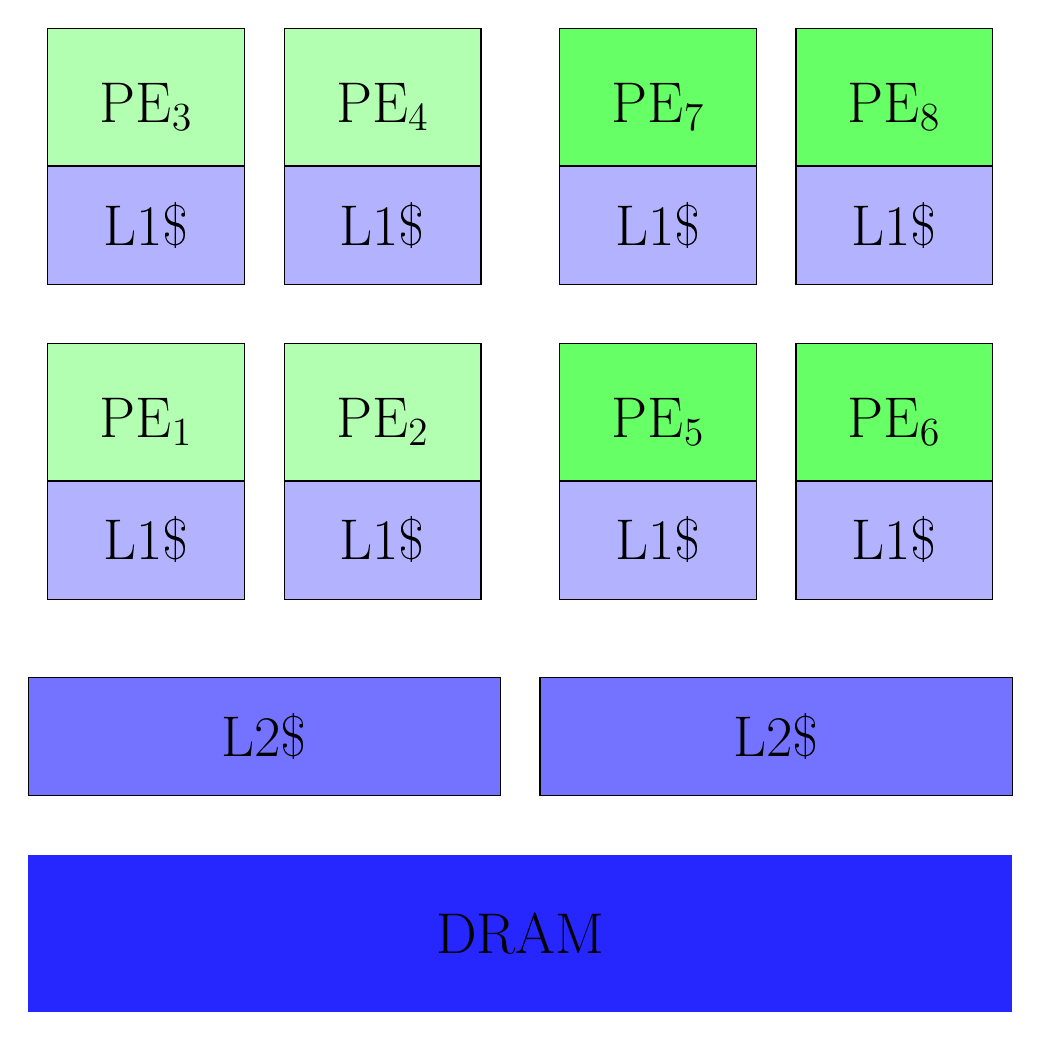
\begin{tikzpicture}
     %little cores
\node (pe1) at ({-1.5},{4}) [draw,minimum width=2.5cm,align=center,minimum height=2cm, fill=green!30] {\huge PE$_1$};
\node (L1-pe1) at (-1.5,2.5) [draw,minimum width=2.5cm,align=center,minimum height=1.5cm, fill=blue!30] {\huge L1\$};
\node (pe2) at (-1.5+3,4) [draw,minimum width=2.5cm,align=center,minimum height=2cm, fill=green!30] {\huge PE$_2$};
\node (L1-pe2) at (-1.5+3,2.5) [draw,minimum width=2.5cm,align=center,minimum height=1.5cm, fill=blue!30] {\huge L1\$};
\node (pe3) at (-1.5,4+4) [draw,minimum width=2.5cm,align=center,minimum height=2cm, fill=green!30] {\huge PE$_3$};
\node (L1-pe3) at (-1.5,2.5+4) [draw,minimum width=2.5cm,align=center,minimum height=1.5cm, fill=blue!30] {\huge L1\$};
\node (pe4) at (-1.5+3,4+4) [draw,minimum width=2.5cm,align=center,minimum height=2cm, fill=green!30] {\huge PE$_4$};
\node (L1-pe4) at (-1.5+3,2.5+4) [draw,minimum width=2.5cm,align=center,minimum height=1.5cm, fill=blue!30] {\huge L1\$};

%big cores
\node (pe5) at ({6.5-1.5},{4}) [draw,minimum width=2.5cm,align=center,minimum height=2cm, fill=green!60] {\huge PE$_5$};
\node (L1-pe5) at (6.5-1.5,2.5) [draw,minimum width=2.5cm,align=center,minimum height=1.5cm, fill=blue!30] {\huge L1\$};
\node (pe6) at (6.5-1.5+3,4) [draw,minimum width=2.5cm,align=center,minimum height=2cm, fill=green!60] {\huge PE$_6$};
\node (L1-pe6) at (6.5-1.5+3,2.5) [draw,minimum width=2.5cm,align=center,minimum height=1.5cm, fill=blue!30] {\huge L1\$};
\node (pe7) at (6.5-1.5,4+4) [draw,minimum width=2.5cm,align=center,minimum height=2cm, fill=green!60] {\huge PE$_7$};
\node (L1-pe7) at (6.5-1.5,2.5+4) [draw,minimum width=2.5cm,align=center,minimum height=1.5cm, fill=blue!30] {\huge L1\$};
\node (pe8) at (6.5-1.5+3,4+4) [draw,minimum width=2.5cm,align=center,minimum height=2cm, fill=green!60] {\huge PE$_8$};
\node (L1-pe8) at (6.5-1.5+3,2.5+4) [draw,minimum width=2.5cm,align=center,minimum height=1.5cm, fill=blue!30] {\huge L1\$};


\node (L2-little) at (0,0) [draw,minimum width=6cm,align=center,minimum height=1.5cm, fill=blue!55] {\huge L2\$};
\node (L2-big) at (6.5,0) [draw,minimum width=6cm,align=center,minimum height=1.5cm, fill=blue!55] {\huge L2\$};
\node (DRAM) at (3.25,-2.5) [minimum width=12.5cm,align=center,minimum height=2cm, fill=blue!85] {\huge DRAM};
   \end{tikzpicture}
 }
   \caption{Symmetries in the Odroid-XU4 architecture. TODO: fix figure.}
   \label{fig:exynos_symmetries}
\end{figure}

When the memory subsystem is more complex, this is also reflected in the topology. Consider the \ac{NoC}-based architecture depicted in the example, with four identical cores $\PE_1\ldots,\PE_4$.
An analogous transformation to the one described before, which swaps the cores $\PE_1$ and $\PE_2$, is not a symmetry of this topology, as depicted in Figure~\ref{fig:non_equivalent}.
The change in the cores changes the communication patterns.
Before the transformation, sending data from $\PE_1$ to $\PE_3$ needs two hops over the \ac{NoC}, whereas after the transformation it can be sent within a single hop.

\begin{figure}[h]
	\centering
\resizebox{0.3\textwidth}{!}{
   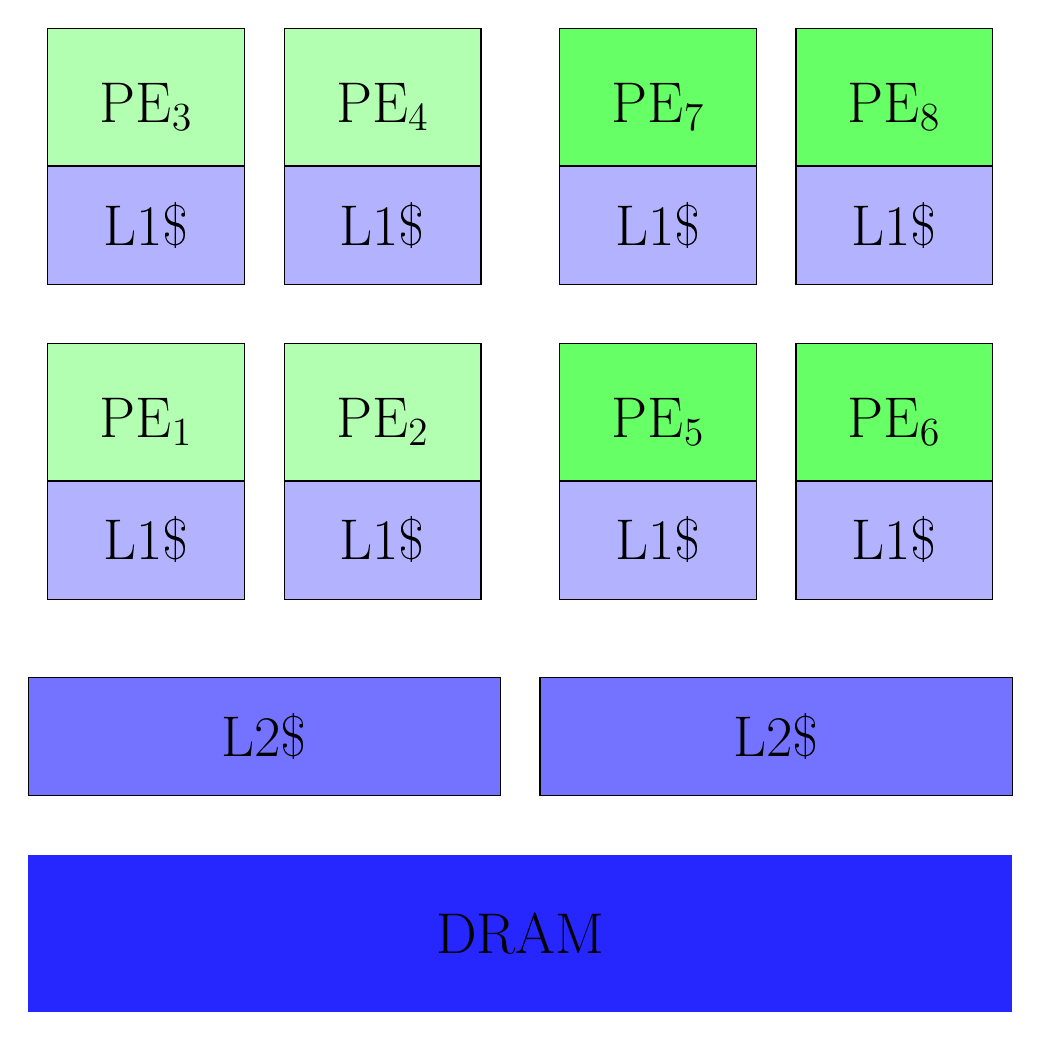
\begin{tikzpicture}
     %little cores
\node (pe1) at ({-1.5},{4}) [draw,minimum width=2.5cm,align=center,minimum height=2cm, fill=green!30] {\huge PE$_1$};
\node (L1-pe1) at (-1.5,2.5) [draw,minimum width=2.5cm,align=center,minimum height=1.5cm, fill=blue!30] {\huge L1\$};
\node (pe2) at (-1.5+3,4) [draw,minimum width=2.5cm,align=center,minimum height=2cm, fill=green!30] {\huge PE$_2$};
\node (L1-pe2) at (-1.5+3,2.5) [draw,minimum width=2.5cm,align=center,minimum height=1.5cm, fill=blue!30] {\huge L1\$};
\node (pe3) at (-1.5,4+4) [draw,minimum width=2.5cm,align=center,minimum height=2cm, fill=green!30] {\huge PE$_3$};
\node (L1-pe3) at (-1.5,2.5+4) [draw,minimum width=2.5cm,align=center,minimum height=1.5cm, fill=blue!30] {\huge L1\$};
\node (pe4) at (-1.5+3,4+4) [draw,minimum width=2.5cm,align=center,minimum height=2cm, fill=green!30] {\huge PE$_4$};
\node (L1-pe4) at (-1.5+3,2.5+4) [draw,minimum width=2.5cm,align=center,minimum height=1.5cm, fill=blue!30] {\huge L1\$};

%big cores
\node (pe5) at ({6.5-1.5},{4}) [draw,minimum width=2.5cm,align=center,minimum height=2cm, fill=green!60] {\huge PE$_5$};
\node (L1-pe5) at (6.5-1.5,2.5) [draw,minimum width=2.5cm,align=center,minimum height=1.5cm, fill=blue!30] {\huge L1\$};
\node (pe6) at (6.5-1.5+3,4) [draw,minimum width=2.5cm,align=center,minimum height=2cm, fill=green!60] {\huge PE$_6$};
\node (L1-pe6) at (6.5-1.5+3,2.5) [draw,minimum width=2.5cm,align=center,minimum height=1.5cm, fill=blue!30] {\huge L1\$};
\node (pe7) at (6.5-1.5,4+4) [draw,minimum width=2.5cm,align=center,minimum height=2cm, fill=green!60] {\huge PE$_7$};
\node (L1-pe7) at (6.5-1.5,2.5+4) [draw,minimum width=2.5cm,align=center,minimum height=1.5cm, fill=blue!30] {\huge L1\$};
\node (pe8) at (6.5-1.5+3,4+4) [draw,minimum width=2.5cm,align=center,minimum height=2cm, fill=green!60] {\huge PE$_8$};
\node (L1-pe8) at (6.5-1.5+3,2.5+4) [draw,minimum width=2.5cm,align=center,minimum height=1.5cm, fill=blue!30] {\huge L1\$};


\node (L2-little) at (0,0) [draw,minimum width=6cm,align=center,minimum height=1.5cm, fill=blue!55] {\huge L2\$};
\node (L2-big) at (6.5,0) [draw,minimum width=6cm,align=center,minimum height=1.5cm, fill=blue!55] {\huge L2\$};
\node (DRAM) at (3.25,-2.5) [minimum width=12.5cm,align=center,minimum height=2cm, fill=blue!85] {\huge DRAM};
   \end{tikzpicture}
 }
   \caption{The communication topology affects symmetries in architectures.}
   \label{fig:non_equivalent}
\end{figure}

Generally, the transformations that preserve the structure of the architecture topology have a clear structure.
If two transformations $t_1$ and $t_2$ preserve the structure of the architecture topology, then their composition $t_1 \circ t_2$ also preserves it.
Similarly, it is clear that reversing a transformation $t_1^{-1}$ also preserves the structure.
Finally, the identity transformation on the architecture $\operatorname{id}_A$ (which does not change anything) clearly preserves the structure.
These observations together mean that these transformations have the structure of a group with the function composition $(\circ)$ as its operation.

More precisely, the group of symmetries of the achitecture is precisely the group of graph isomorphisms from the architecture graph $A$ to itself.
An isomorphism from an object to itself is called an automorphism\index{automorphism}.
We denote the group of automorphisms of the architecture $A$ as $\Aut(A)$

For the case of the \ac{NoC}-based architecture, the authomorphism group $\Aut(A\text{NoC}) \cong D_4$ is a dihederal group on $4$ points.
It conists of $3$ rotations, $4$ reflections and the identity transformation.
The Odroid architecture, on the other hand, has $\Aut(A_\text{Odroid}) \cong S_4 \times S_4$ as symmetry group.
This group with $48$ transformations is comprised of (independent) arbitrary permutations of the A15 and A7 cores.

Since the Odroid architecture is heterogeneous, both clusters are distinct and there is no symmetry between them.
Many complex architectures, however, do consist of multiple identical culsters. Consider the architecture depicted in Figure~\ref{fig:coolidge}.
It is the MPPA3 Coolidge from Kalray~\cite{coolidge} and consists of $5$ identical clusters.
Each cluster has $17$ cores, $16$ of which are identical general-purpose cores, and the last one is a special-purpose secure and management core.

The MPPA3 Coolidge is a hierarchically-designed architecture. The five identical clusters are conceptually at a different level than the cores at each cluster.
Designs like the HAEC~\cite{haec} topology mentioned in the introduction (cf. Figure~\ref{fig:haec}) have even more levels of hierarchy.
The symmetries of these hierarchical architectures are reflected in the different levels of hierarchy of the topology~\cite{goens_tcad21}.
For example, the automorphism group of the MPPA3 Coolidge is $\Aut(A_\text{Coolidge}) \cong S_{16} \wr S_5$ and has $16! \cdot 5! \approx 2.51 \cdot 10^{15}$ symmetries. 

So far we have discussed the symmetries of architectures.
However, we can apply the same principle to applications and their graphs.
Conisder the audio filter example application from Section~\ref{sec:kpn_basic} (cf. Figure~\ref{fig:audio_filter_graph}). 
The left and right channels perform precisely the same computation on different data.
We could not, for example, just swap the \texttt{fft\_l} and \texttt{fft\_r} nodes, since that would result in a different application that also swaps the channels of the audio file.
On the other hand, if we swap the whole subgraph consisting of \texttt{fft\_l}, \texttt{filter\_l} and \texttt{ifft\_l} with the equivalent subgraph of \texttt{fft\_r}, \texttt{filter\_r} and \texttt{ifft\_r}, the application remains identical.
This is depicted on Figure~\ref{fig:audio_filter_symmetries}.

\begin{figure}[h]
	\centering
\resizebox{0.9\textwidth}{!}{
\begin{tikzpicture}
   \node[draw, ellipse,minimum width = 1.1cm, minimum height=0.9cm] (src) {src};
\node[draw, ellipse,minimum width = 1.1cm, minimum height=0.9cm, below right = 1cm of src] (fft_l) {\texttt{fft\_l}};
\node[draw, ellipse,minimum width = 1.1cm, minimum height=0.9cm, above right = 1cm of src] (fft_r) {\texttt{fft\_r}};
\node[draw, ellipse,minimum width = 1.1cm, minimum height=0.9cm, right = 1 cm of fft_l] (filter_l) {\texttt{filter\_l}};
\node[draw, ellipse,minimum width = 1.1cm, minimum height=0.9cm, right = 1 cm of fft_r] (filter_r) {\texttt{filter\_r}};
\node[draw, ellipse,minimum width = 1.1cm, minimum height=0.9cm, right = 1 cm of filter_l] (ifft_l) {\texttt{ifft\_l}};
\node[draw, ellipse,minimum width = 1.1cm, minimum height=0.9cm, right = 1 cm of filter_r] (ifft_r) {\texttt{ifft\_r}};
\node[draw, ellipse,minimum width = 1.1cm, minimum height=0.9cm, below right = 1cm of ifft_r] (sink) {\texttt{sink}};

\draw[-latex] (src) -- (fft_l);
\draw[-latex] (src) -- (fft_r);
\draw[-latex] (fft_l) -- (filter_l);
\draw[-latex] (fft_r) -- (filter_r);
\draw[-latex] (filter_l) -- (ifft_l);
\draw[-latex] (filter_r) -- (ifft_r);
\draw[-latex] (ifft_l) -- (sink);
\draw[-latex] (ifft_r) -- (sink);
 \end{tikzpicture}
}
   \caption{A symmetry of the audio filter application. TODO: adapt figure}
	\label{fig:audio_filter_symmetries}
\end{figure}

Mathematically, we need to model the semantics of the application to reflect its symmetries.
For an application $K = (V_K,E_K)$ we can label the nodes $V_K$ with unique identifiers relating them to the $KPN$ process that execute them (e.g. the \texttt{\_\_PNprocess} in a \ac{CPN} program). 
Formally, thus, the automorphism group $\Aut(E)$ of the labeled graph $K$ is trivial, i.e. $\Aut(E) = \{ \id \}$. 
We could label $K$ differently to capture the symmetry from Figure~\ref{fig:audio_filter_symmetries}.
For example, if use the source code of the process as label, we would capture this symmetry.
We have to be more careful, however, as this can lead to a problematic definition of symmetries.

An application might use the same code at different points, resulting in very different behavior.
For example, consider an application that receives a list of points, which it sorts before operating on it.
Before returning the list, it sorts them again to ensure they are sorted.
Both times it sorts the list using the quicksort algorithm, yet the second time the list is almost always sorted or close to being sorted.
Then the execution of the same quicksort code in the second instance behaves very differently from the first time.

A difference like the one outlined above is very difficult to capture automatically, as it requires understanding of the application to a very high level of abstraction.
We thus consider application symmerties as manually-defined anotations.
There are some conceivable ways to automatically capture and annotate such application symmetries, for example when dealing with known data-level parallelism.
In future work, a framework as we discuss in Chapter~\ref{chap:mocs}, Section~\ref{sec:macqueen} could be extended to extract symmetries.
For the rest of this thesis, however, we focus on symmetries induced from the architecture.

\subsection{Mappings}

We have seen how the architecture and applications have symmetries in their structure. 
The groups $\Aut(A)$ and $\Aut(K)$ act on the architecture $A$ and the application $K$, respectively.
These actions also induce an action on the mapping space. 
Let $m : K \rightarrow A$ be a mapping.
Recall that a symmetry $\sigma \in \Aut(A)$ of the architecture is a transformation that leaves the structure of the architecture unchanged.
Conisder then the mapping $\sigma m := k \mapsto \sigma(m(k))$.
Since the structure of $A$ is unchanged, then the structure of $m$ and $\sigma m$ is also identical.
All observable properties of $m$ and $\sigma m$, like the execution time or energy consumption, are the same.
If they were not, it would have to be due to a structural difference in the (sub)architectures $m(K),(\sigma m)(k) = \sigma(m(K)) \leq A$, which are isomorphic by assumption on $\sigma$.
We say that these properties like the execution time and energy consumption are \emph{invariants}\index{invariants} of the group action.

Figure~\ref{fig:mapping_action_example} shows an example of the action on mappings. \todo{add and describe figure.}

The case for $K$ is analogous.
Let $\pi \in \Aut(K)$ be a symmetry of the application.
Then the mapping $\pi m := k \mapsto m(\pi^{-1}k)$ is equivalent to $m$.
Note that we define it with $\pi^{-1}$ instead of $\pi$ so that this defines a left action.
Indeed, for $\pi, \tau \in \Aut(K)$, we have
\begin{align*}
  (\pi (\tau m))(k) = \pi m(\tau^{-1}k) = m(\pi^{-1}\tau^{-1}k) = m((\tau \pi)^{-1}k) = ((\tau \pi) m))(k) 
\end{align*}

From the models of the problem, as defined in Chapter~\ref{chap:mapping}, mappings under these symmetries are necessarily indistinguishable from each other, since they rely on inherent symmetries of the models.
On the other hand, these are just models, they need not reflect reality.
It still leaves the question open, how does this hold up in pracitice?
Are equivalent mappings actually equivalent?
In~\cite{goens_scopes17} we tested this empirically, by executing four equivalent mappings and measuring the runtime and energy.
We tested four equivalent mappings of the audio filter benchmark on an Odroid XU3 and executed each $50$ times, measuring three metrics.
The Odroid XU3 is almost identical to the Odroid XU4, but features on-board energy sensors.
We measured the \acs{CPU} time, which is the total aggregate time spent by all \acsp{CPU} executing the application.
We also measured the wall-clock time, which is the total time of the application, measured from start to finish as it would pass on a wall clock.
Finaly, we measured the total energy over the INA-231 sensors connected over the I2C bus, as the aggregate of the energy measured at each individual component, sampled at $10$~Hz.

\begin{figure}[h]
	\centering
\resizebox{0.95\textwidth}{!}{
     \input{generated/mappings_equivalent}
 }
   \caption{Measurements of four equivalent mapings for the audio filter application on the Odroid-XU3 architecture.}
   \label{fig:symmetry_measurements}
\end{figure}

Figure~\ref{fig:symmetry_measurements} shows the results of the measurements as box-and-whiskers plots.
We see that the execution times of all mappings are well within the ranges of each other, both when measured as wall-clock or \ac{CPU} time.
We can test this in a more rigurous fashion with an \ac{ANOVA} F-test.
For the wall-clock data, we get a probability of $p = 5.06\%$, rejecting the null hypothesis that variance in the wall-clock times from different mappings is explained by more than statistical variance.
For the \ac{CPU} time data, the value of $p=15.2\%$ it is even clearer that the variance is likely just statistical.
We can conclude that, at least for this example, equivalent mappings indeed seem to have the same execution time behavior.

The energies of the mappings are less clearly distinct, especially for the first two mappings, yet they all still require comparable amounts of erengy.
An \ac{ANOVA} F-test yields a $p$ value of $0.009\%$.
It is worth noting here that these measurements are just a first estimation.
The accuracy of the energy data depends on a multitude of factors like the sampling rate or the measurement accuracy of the INA-231 sensors.
We have not made a proper assesment of measurement errors and error propagation, which is especially large in the energy measurements that span measurements from four different components.
Precise energy measurments, however, are beyond the scope of this thesis.
We this experiment we cannot really conclude nor discard the hypothesis that energy consumption is an invariant of the mapping symmetries.

\subsection{Calculating Symmetries}

The branch of mathematics known as computational group theory deals with computational aspects of the theory of groups, which we have used here for formalizing the symmetries of applications, architectures and mappings. 
An overview of the methods of computational group theory can be found in~\cite{seress2003permutation} covering beyond the basics presented in this subsection.
Here we will present only the methods necessary for the calculations required of applications to software synthesis.

To leverage the symmetries explained in this theses for software synthesis, we need to methods to calculate the following:
\begin{itemize}
\item Given an architecture graph $A$, the group of symmetries $\Aut(A)$.
\item Given a mapping $m : T \rightarrow A$ and the symmetry group $G := \Aut(T \rightarrow A)$, enumerate the orbit $Gm$.
\item Given two mappings $m,m' : T \rightarrow A$ and the symmetry group $G := \Aut(T \rightarrow A)$, determine wether $m = gm'$ for a $g \in G$, i.e. if the two mappings are in the same orbit.
\end{itemize}


\subsection{Partial Symmetries}

The symmetries we have considered so far can be considered as ``global'' symmetries: they are transformations of the complete structure (e.g. architecture, mapping).
The intuitive notion of symmetry, however, is more general than this. What we consider as symmetry also inlcludes the relationship of as tructure to each parts.
In particular, a symmetry can be local to a part of the structure, without being global. A general discussion of this can be found in~\cite{lawson_inverse_semigroups}, as well as a detailed exposition of the mathematical background of this section.

We can see what we mean by local structures in the example depicted in Figure~\ref{fig:motivation_partial_symmetries}.
It shows two \ac{NoC} architectures both with a regular mesh topology.
The first one is a two-by-two mesh, the second one four-by-four.
We can compare now the symmetries of both architectures intuitively, and see how these translate to the group-theoretic sense.
The four-by-four mesh is larger, and has a sort of self-similarity: it can be thought of as composed of four copies of the two-by-two mesh arranged in a larger two-by-two mesh.
Intuitively, thus, this four-by-four mesh has more symmetry.

\begin{figure}[h]
	\centering
   \resizebox{0.55\textwidth}{!}{\begin{tikzpicture}
\draw (0,0) rectangle (5,5);
\draw (2.5,2.5) node {Placeholder};
\end{tikzpicture}
}
	\caption{A comparison of the symmetries of two meshes.}
	\label{fig:motivation_partial_symmetries}
\end{figure}

However, if we look at the group of automorphisms of the corresponding architecture graphs, we get a result that defies this intuition:
both archtiectures have the same groups of symmetries!
More precisely, their groups of automorphisms are isomorphic, they are dihederal groups on 4 points, $D_4$.
More concretely, there are only 8  possible structure-preserving transformations acting on these two topologies, which are the rotations of $90^\circ,180^\circ,270^\circ,360^\circ = 0^\circ$ and the reflections among each of the axes (horizontal, vertical and both diagonals). We cannot, for example, divide the four-by-four mesh into a two-by-two mesh of two-by-two meshes, and rotate that larger two-by-two mesh by $90^\circ$ or one of the smaller ones by $90^\circ$. These two operations both work locally, if we ignore the rest of the structure, but do not preserve the whole structure of the mesh, as illustrated by Figure~\ref{fig:partial_symmetries_4x4}.

\begin{figure}[h]
	\centering
   \resizebox{0.55\textwidth}{!}{\begin{tikzpicture}
\draw (0,0) rectangle (5,5);
\draw (2.5,2.5) node {Placeholder};
\end{tikzpicture}
}
	\caption{Some partial symmetries of a 4x4 mesh.}
	\label{fig:partial_symmetries_4x4}
\end{figure}

For the mathematical formalization of this intuitive notion of local symmetries, in this section, we follow~\cite{lawson_inverse_semigroups}.
There are essentially two ways equvialent ways of formalizing this intuitive notion of local symmetries, inverse semigroups and ordered groupoids.
We will consider the formalization using inverse semigroups, as it is conceptually simpler for computations, and mathematically equally as powerful.
In the case of global symmetries there are concrete trasformations of architectures and mappings and corrpesponding abstract groups. For partial symmetries we will consider partial trasformations of mappings which we will model as partial permutations, and these partial permutations (transformations) have a corresponding abstract inverse semigroup.

We start by defining partial functions and partial permutations.
\begin{defn}
Let X,Y be sets.
A \emph{partial function} $f: X \rightarrow Y$ is a function from a subset of $X$ to a subset of $Y$.
We denote the domain of by $\dom(f)$ the codomain of $f$ by $\cod(f)$.
Thus, the partial function $f: X \rightarrow Y$ is a (total) function $f: \dom(f) \rightarrow \cod(f)$
\end{defn}

\begin{defn}
Let $X$ be a set.
A partial function $f: X \rightarrow X$ from $X$ to itself is called a \emph{partial permutation} if the (total) function $f: \dom(f) \rightarrow \cod(f)$ is a bijection between $\dom(f)$ and $\cod(f)$.
\end{defn}

\begin{figure}[h]
	\centering
   \resizebox{0.55\textwidth}{!}{\begin{tikzpicture}
\draw (0,0) rectangle (5,5);
\draw (2.5,2.5) node {Placeholder};
\end{tikzpicture}
}
	\caption{An example of a partial permutation in a $4 \times 4$ mesh.}
	\label{fig:example_partial_permutation}
\end{figure}

We can think of partial functions thus as functions that are not defined everywhere, and partial permutations, acordingly, are not defined everywhere.
For example, the partial permutation $f : \{0,\ldots,15\} \rightarrow \{0,\ldots,15\}$ defined as $f(0) = 4, f(1) = 0, f(4) = 5, f(5) = 1$ is a rotation of the upper-left $2 \times 2$-mesh in the $4\times 4$-mesh, but is not defined on the rest of the architecure. This is a partial symmetry of the $4\times 4$-mesh. This partial permutation is dpeicted in Figure~\ref{fig:example_partial_permutation}. We can write it also as:
\begin{equation*}
\left(
\begin{array}{llllllllllllllll}
0 & 1 & 2 & 3 & 4 & 5 & 6 & 7 & 8 & 9 & 10 & 11 & 12 & 13 & 14 & 15\\
4 & 0 & - & - & 5 & 1 & - & - & - & - &  - &  - &  - &  - &  - &  -
\end{array}
\right)
\end{equation*}
Because the set $\{0,\ldots,15\}$ is understood from context, we can also write it, shorter, as:
\begin{equation*}
\left(
\begin{array}{llll}
0 & 1 & 4 & 5 \\
4 & 0 &  5 & 1
\end{array}
\right)
\end{equation*}

We also use a notation similar to the cycle notation of group theory, where we use a cicle with round brackets to denote a full cycle, where the last element maps to the first.
Square brackets to denote when this is not the case, i.e. the function is not defined on the last element of that cycle. In this notation, singleton cycles cannot be omitted as in the case of groups.
In other words, fixed points have to be represented as one-element cycles.
The partial permutation from Figure~\ref{fig:example_partial_permutation} can thus be written much more compactly as: $(0,4,5,1)$.
This is a full cycle, but it is only defined on the subset $\{0,1,4,5\}$.
In the group context, the cycle $(0,4,5,1)$ as an element of the symmetric group on 15 points, would instead mean the (complete) permutation that fixes $\{2,3,6,7,8,9,10,11,12,13,14,15\}$.
As a partial permutation in cycle notation we would write this as: \[(0,4,5,1)(2)(3)(6)(7)(8)(9)(10)(11)(12)(13)(14)(15) \]
A different example of a partial permutation is the partial permutation that moves the first row to the right (and is not defined on the rest), as a cycle: $[0,1][4,5][8,9][12,13]$.
On the other hand, the partial permutation that is a diagonal reflection on the upper-left $2 \times 2$ (sub)mesh is, in cycle notation, $(1,4)(0)(5)$.
These two partial permutations can also be written in the matrix notation from above as:

\begin{equation*}
\left(
\begin{array}{llll}
0 & 4 & 8 & 12 \\
1 & 5 & 9 & 13 
\end{array}
\right)
\quad
\left(
\begin{array}{llll}
0 & 1 & 4 & 5 \\
0 & 4 & 1 & 5
\end{array}
\right)
\end{equation*}

For computations~\cite{east2019semigroups}, the three notations can be interpreted to make different data structures that make different opperations more efficient, like application of the partial function (as an array look-up), for sparse partial permutations (as lookups in key-value pairs), or cycles for efficient multiplication (as concatenation). They have different benefits and drawbacks. For readability though, the cycle notation is the most compact one, and the one we will use for the rest of this thesis.

Just as for groups, we can define the (left) action of a semigroup:
\begin{defn}
Let $S$ be a semigroup and $X$ be a set. We say that $S$ \emph{acts} on $X$ (on the left) if there is a function $\cdot : S \times X \rightarrow X$ such that $(ab) \cdot x = a \cdot (b \cdot x)$. If $S$ is a monoid with identity $1$ and the function $\cdot$ satisfies the condition $1 \cdot x = x$ for all $x \in X$, we say that the action is a monoid action.
\end{defn}

The action of a semigroup of partial permutations to an architecture works the same as with groups, except it does not work on the whole architecture.
Let $f$ be a partial permutation on an architecture $A$, and $m : T \rightarrow A$ be a mapping on that arcticeture.
If the partial permutation is defined on all cores mappend on by $m$, i.e., $im(m) \subseteq \dom(f)$, then we can use the action of the semigroup of partial permutations of $A$ to define another mapping $fm$ by $fm(t) = f \cdot m(t)$
for all $t$ in $T$. If $f$ is not defined on some of the cores of $m$, i.e., $im(m) \not \subseteq \dom(f)$, then we cannot define $fm$. In this way, $f$ also defines a partial permutation $\hat f$ on the set of mappings $\{ m : T \rightarrow A \}$.
\todo{check that notation is consistent}

Consider for example the mapping of an application with three tasks to the $4 \times 4$-mesh defined by $m_0(t_0) = m_0(t_2) = \PE_0$ and $m_0(t_1) = \PE_1$, which we can also write as the vector $m_0 = (0,1,0)$.
Then the partial permutation $(0,4,5,1)$ from Figure~\ref{fig:exapmle_partial_permutation} above defines the mapping $(0,4,5,1)m = (4,0,4)$.
Similarly, the action of the partial permutation $(1,4)(0)(5)$ yields a new mapping, $(1,4)(0)(5)m_0 = (0,4,0)$.
However, since the translation $[0,1][4,5][8,9][12,13]$ is not defined on $1 = m_0(t_1)$, we cannot define $[0,1][4,5][8,9][12,13]$ as a mapping.
Formally we can say that the partial permutations $\widehat{(0,4,5,1)}$ and $\widehat{(1,4)(0)(5)}$ are defined on $m_0$, but $\widehat{[0,1][4,5][8,9][12,13]}$ is not defined on $m_0$.

What happens with application symmetries? Consider ...

Define orbits for inverse semigroups and s.c.c.

We are now ready to formally define the set of partial symmetries of architectures, applications in mappings as in the case of groups.
\begin{defn}
$\AutSemi$
\end{defn}

There is a different way of intperpreting these notions of symmetry, using graph isomorphisms.
Recall that a mapping $m: T \rightarrow A$ can be seen as a morphism of graphs from $T$ to $A$.
In particular, every mapping $m$ defines a subgraph $m(T) \leq A$.
This subraph has a node $m(t) \in V_A$ for every $PE$ in the architecture $A$ that is used in a mapping, and similarly an endge $(m(t_1),m(t_2)) \in E_A$ for every communication primitive where a channel is mapped to.
Figure~\ref{fig:example_graph_isomorphism} shows this graph for two of the mappings discussed above, $m_0 = (0,1,0)$ and $m_1 := (0,4,5,1)m_0 = (4,0,4)$. 
You can see that the architecture subgraphs of the mappings are identical. In fact, if there is a partial symmetry, these two graphs will always be identical:

\begin{figure}[h]
	\centering
   \resizebox{0.55\textwidth}{!}{\begin{tikzpicture}
\draw (0,0) rectangle (5,5);
\draw (2.5,2.5) node {Placeholder};
\end{tikzpicture}
}
	\caption{Some partial symmetries of a 4x4 mesh.}
	\label{fig:partial_symmetries_4x4}
\end{figure}
It is a sort of trace of the mapping. This mapping does not describe 
\todo{check that notation is consistent}

\begin{lem}
\label{lem:symmetry_to_iso}
Let $m : T \rightarrow A$ be a mapping and let $f \in \AutSemi(A)$ be a partial automorphism of the archtitecture such that $\im(m) \subseteq \dom(f)$. Then, the two graphs $m(T)$ and $(fm)(T)$ are isomoprhic and the function $\varphi: m(T) \rightarrow (fm)(T), m(t) \mapsto f \cdot m(t)$ for all $t \in T$ is an isomorphism of labeled graphs.
\begin{proof}
First note that $\varphi$ is well-defined. Indeed, since $\im(m) \subseteq \dom(f)$ it means that $f \cdot m(t)$ is defined for all $t \in T$. Since $f \in \AutSemi(A)$, we know that the type of $m(t)$ and $f \cdot m(t)$ is equal for all $t \in T$, as well as the type of all edges $(m(t_0),m(t_1))$ and  $(f \cdot m(t_0), f \cdot m(t_1))$ is equal. Thus, $\varphi$ is a morphism of labeled graphs. Finally, since $f \in \AutSemi(A)$, we know that $f$ is a partial permutation, and in particular, a bijection between $\dom(f)$ and $\cod(f)$. In particular, $\varphi$ is bijective, and as a bijective morphism of labeled graphs, an isomorphism. 
\end{proof}
\end{lem}

What about the converse, if the subgraphs generated by the mappings are isomorphic, does this mean that there is a (partial) isomorphism of the mappings too? Can we use this to characterize equivalent mappings? 
In general, no.
Consider the subgraph of the mappings $m_2 := (4,4,0)$ and $m_3 := (4,0,0)$. Both these mappings project into isomorphic subgraphs $m_2(T) \cong m_3(T) \cong m_0(T)$, but obviously the mappings are not equivalent.
Even if the subgraphs are isomorphic, the crucial difference is, however, that the mapping $\varphi$ as defined in Lemma~\ref{lem:symmetry_to_iso} is \textbf{not} an isomorphism of (labeled) graphs. 
What if tasks $t_1$ and $t_2$ are equivalent?
In other words,  what if $g = (0)(1,2)$ is a (full) automorphism of the application graph?
Then the mappings $m_0$ and $m_2$ are equivalent (via $g$), but the function $\varphi$ of Lemma~\ref{lem:symmetry_to_iso} is still not an isomoprhism of the subgraphs.
However, we can generalize the function by applying $g$ first, as $\varphi \circ g : m(T) \rightarrow fm(T), m(t) \mapsto (fm \circ g)(t) = (fm)(g(t))$.
This generalization, in fact, yields a full characterization of equvialent mappings through isomorphy of subgraphs.
\begin{thm}
Let $A$ be an architecture with inverse semigroup of automorphisms $S = \AutSemi(A)$ and let $T$ be an application graph with group of automorphsims $G = \Aut(T)$.
For mappings $m,m' : T \rightarrow A$, the following statements are equvialent:
\begin{enumerate}
\item There exists a partial permutation $f \in S$ and a perumtation $g \in G$, such that $\varphi \circ g$ is an isomorphism of labeled graphs.
\item There two mappings are equivalent by symmetries in the orbit of $S \times G$.
\end{enumerate}
\begin{proof}
The implication $(1) \Rightarrow (2)$ follows directly from the definition of $\varphi$ and the action of $S \times G$.
For the implication $(2) \Rightarrow (1)$, since $m$ and $m'$ are in the same s.c.c. of the orbit of $S \times G$, there exists an $x \in S \times G$ such that $m = x \cdot m'$.
We can use the direct product structure of $S \times G$ to decompose $ x = fg$ for $f \in S, g \in G$.
This means that $m = fg \cdot m' = f \cdot (g \cdot m')$.
Applying Lemma~\ref{lem:symmetry_to_iso} on $m$ and $g \cdot m'$ shows that $\varphi \circ g$ is an isomorphism.
\end{proof}
\end{thm}

How do partial symmetries with inverse semigroups compare to (global) symmetries, in the sense of group theory?
We can start with a simple example, of a $2\times 2$ mesh, which we will call $M_2$. The group of symmetries of this architecture, as we have seen, is $D_4$ with $|D_4| = 8$ symmetries.
What about the partial symmetries? It is easy to check that $|\AutSemi(M_2)| = 45$, which is a lot more partial symmetries than global ones! But in fact, comparing the size of the group and the semigroup is misleading.
We can't compare them, as they deal with different objects, functions vs partial functions. For this case of $M_2$, in a sense, we do not get any more symmetries by going to the partial symmetry world.
We can see it through the following argument: the group $\Aut(M_2) \cong D_4$ acts canonically on the power set of $M_2$, $\operatorname{Pow}(M_2)$, simply by acting element-wise:
For $M \subseteq M_2$ and $g \in \Aut(M_2)$, the (canonical) action is defined as follows: $g \cdot M := \{ g \cdot m \mid m \in M \}$.
In this action, the orbits $G \\ \operatorname{Pow}(M_2)$ are in obvious bijection to the s.c.c. of the orbit of $\AutSemi(M_2) \\ \operatorname{M_2}$.
Concretely




\subsection{Calculating Semigroups of Symmetries}

Now that we have seen how to describe partial symmetries, we can proceed to explain how to calculate them.
This subsection is a simplification of the methods of~\cite{east2019semigroups}, and our applications of it in joint work with S. Siccha and J. Castrillon~\cite{goens_taco17}.
